% file: BLT_5_poset_lvl_6_draw.tex
% created by Orbiter tikz interface
% creation date: Tue Dec 22 00:05:02 MST 2020
% DeviceCoordinates 0 0 1000000 1000000
% UserCoordinates 0 0 10000 10000
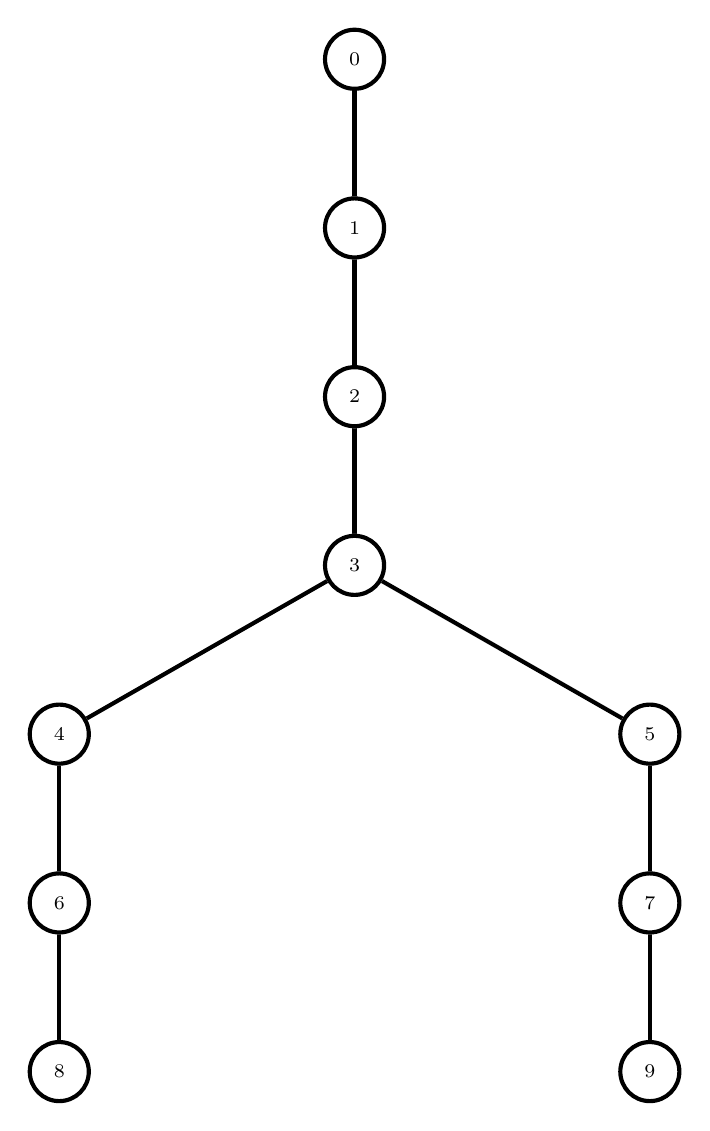
\begin{tikzpicture}[scale=0.45,line width = 1.5pt]
\draw [] (16.6667,30.95) -- (16.6667,26.19);
\draw [] (16.6667,26.19) -- (16.6667,21.4267);
\draw [] (16.6667,21.4267) -- (16.6667,16.6667);
\draw [] (16.6667,16.6667) -- (8.33333,11.9033);
\draw [] (16.6667,16.6667) -- (25,11.9033);
\draw [] (8.33333,11.9033) -- (8.33333,7.14);
\draw [] (25,11.9033) -- (25,7.14);
\draw [] (8.33333,7.14) -- (8.33333,2.38);
\draw [] (25,7.14) -- (25,2.38);
\filldraw[color=white] (16.6667,30.95) circle [radius = 0.833333cm];
\draw (16.6667,30.95) circle [radius = 0.833333cm];
\draw (16.6667,30.95) node{{\scriptsize 0}};
\filldraw[color=white] (16.6667,26.19) circle [radius = 0.833333cm];
\draw (16.6667,26.19) circle [radius = 0.833333cm];
\draw (16.6667,26.19) node{{\scriptsize 1}};
\filldraw[color=white] (16.6667,21.4267) circle [radius = 0.833333cm];
\draw (16.6667,21.4267) circle [radius = 0.833333cm];
\draw (16.6667,21.4267) node{{\scriptsize 2}};
\filldraw[color=white] (16.6667,16.6667) circle [radius = 0.833333cm];
\draw (16.6667,16.6667) circle [radius = 0.833333cm];
\draw (16.6667,16.6667) node{{\scriptsize 3}};
\filldraw[color=white] (8.33333,11.9033) circle [radius = 0.833333cm];
\draw (8.33333,11.9033) circle [radius = 0.833333cm];
\draw (8.33333,11.9033) node{{\scriptsize 4}};
\filldraw[color=white] (25,11.9033) circle [radius = 0.833333cm];
\draw (25,11.9033) circle [radius = 0.833333cm];
\draw (25,11.9033) node{{\scriptsize 5}};
\filldraw[color=white] (8.33333,7.14) circle [radius = 0.833333cm];
\draw (8.33333,7.14) circle [radius = 0.833333cm];
\draw (8.33333,7.14) node{{\scriptsize 6}};
\filldraw[color=white] (25,7.14) circle [radius = 0.833333cm];
\draw (25,7.14) circle [radius = 0.833333cm];
\draw (25,7.14) node{{\scriptsize 7}};
\filldraw[color=white] (8.33333,2.38) circle [radius = 0.833333cm];
\draw (8.33333,2.38) circle [radius = 0.833333cm];
\draw (8.33333,2.38) node{{\scriptsize 8}};
\filldraw[color=white] (25,2.38) circle [radius = 0.833333cm];
\draw (25,2.38) circle [radius = 0.833333cm];
\draw (25,2.38) node{{\scriptsize 9}};
\end{tikzpicture}
